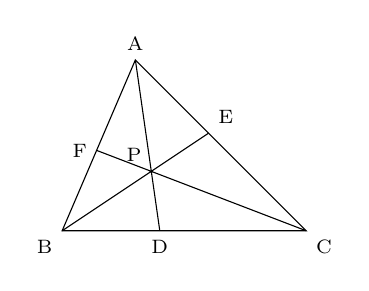
\begin{tikzpicture}[scale=0.62]
\coordinate (B) at (0,0); \coordinate (C) at (5,0); \coordinate (A) at (1.5,3.5);
\coordinate (D) at (2,0); \coordinate (E) at (3,2); \coordinate (F) at (0.706,1.647); \coordinate (P) at (1.826,1.217);
\draw (A)--(B)--(C)--cycle; \draw (A)--(D) (B)--(E) (C)--(F);
\node[above] at (A){\scriptsize A}; \node[below left] at (B){\scriptsize B}; \node[below right] at (C){\scriptsize C};
\node[below] at (D){\scriptsize D}; \node[above right] at (E){\scriptsize E}; \node[left] at (F){\scriptsize F}; \node[above left] at (P){\scriptsize P};
\end{tikzpicture}